\section{Basic Python structures}
	\subsection{Basic Maths}
You can just start typing maths into Python and it will do it.
		\begin{lstlisting}[language=Python]
1+2\end{lstlisting}
		\begin{verbatim}> 3\end{verbatim}
		
Division in Python 3 gives a decimal answer as you would expect.
		\begin{lstlisting}[language=Python]
5/2\end{lstlisting}
		\begin{verbatim}> 2.5\end{verbatim}

		Beware the division operator in Python 2 (you should all be using Python 3!). The above would give an integer division and so return an answer of 2.
		
		The symbol for power is a double star. A square root can be achieved by raising to the power of 1/2.
		\begin{lstlisting}[language=Python]
2**3\end{lstlisting}
		\begin{verbatim}> 8\end{verbatim}

	\subsection{Variables}\label{types}
		We can store values in variables. You can think of these as ``buckets'' which hold values. You can call variables anything you like as long as it doesn't start with a number. In addition it is a bad idea to use variable names that are reserved keywords elsewhere in Python such as \texttt{print}, \texttt{sum} or \texttt{list}. 
		\begin{lstlisting}[language=Python]
a = 6 + 3
print(a)
dead_parrot = "This parrot is no more! He has ceased to be!"
print(dead_parrot)\end{lstlisting}
		\begin{verbatim}> 9
			> This parrot is no more! He has ceased to be!
		\end{verbatim}
		Variables have types. The main types you need to worry about are integers, floats and strings. Integers are whole numbers, floats are decimals and strings are text. Operations between floats and integers are permitted and the answer will be expressed as a float.
		\begin{lstlisting}[language=Python]
spam = 7
eggs = 0.5
food = spam+eggs
print(food)
\end{lstlisting}
		\begin{verbatim}> 7.5\end{verbatim}	
		Operations between strings and number types are generally not permitted since they make no sense.
		\begin{lstlisting}[language=Python]
song = "I'm a lumberjack and I'm OK" + 1\end{lstlisting}
		\begin{verbatim}> TypeError                                 Traceback (most recent call last)
<ipython-input-47-84d795fdab55> in <module>()
----> 1 "I'm a lumberjack and I'm OK" + 1

TypeError: cannot concatenate 'str' and 'int' objects\end{verbatim}

Strings can be concatenated though using the plus symbol.	
		\begin{lstlisting}[language=Python]
line_one = "I'm a lumberjack and I'm OK, "
line_two = "I work all night and I work all day"
song = line_one + line_two
print(song)\end{lstlisting}
		\begin{verbatim}> 9
			> "I'm a lumberjack and I'm OK, I work all night and I work all day"
		\end{verbatim}

	\subsection{Lists}
	Lists are a simple data structure that allow the storage of multiple values. Lists are designated by square brackets. Lists are just another type of variable, so as before you can name them anything you like as long as it doesn't start with a number or is a reserved command (like print).
		\begin{lstlisting}[language=Python]
numberlist = [1, 2, 5]
print(numberlist)\end{lstlisting}
		\begin{verbatim}> [1, 2, 5]\end{verbatim}
		You can fetch a single value from a list by subscripting the list. You can fetch multiple values by asking for a range.
		
		\begin{lstlisting}[language=Python]
numberlist = [1, 2, 3, 4, 5, 6, 7]
print(numberlist[4])
print(numberlist[0:3])\end{lstlisting}
		\begin{verbatim}> [5]
			> [1, 2, 3]
		\end{verbatim}
		Notice how the first command returns 5. This is because Python lists (and many things in programming) start counting at zero. This means asking for the zeroth element would return 1.
		The second command returns only three values. This is because the lower bound is inclusive but the upper bound is exclusive (for mostly the same reasons that things start counting at zero not one). 
		The append command will add things onto the end of a list.
		\begin{lstlisting}[language=Python]
numberlist.append(8)
print(numberlist)	\end{lstlisting}
		\begin{verbatim}> [1, 2, 5, 8]\end{verbatim}
	\subsection{User input}
		Somtimes it is useful to accept some user input while the program is running and operate on this input. This can be achieved with the input command.
		\begin{lstlisting}[language=Python]
person_name = input("What is your name?")
print("Hello " + person_name)\end{lstlisting}
		\begin{verbatim}> Hello Arthur Pewty\end{verbatim}
		Note that the input function always interprets the user's input as text. This means that if the input needs to be interpreted as a number then it should be converted explicitly to an integer or float using int() or float()
		\begin{lstlisting}[language=Python]
user_input_number = float(input("Enter a number of years: "))
print("Two more than your number is: ", user_input_number+2)\end{lstlisting}
		\begin{verbatim}> Two more than your number is: 42\end{verbatim}

	\subsection{Flow control}
		\subsubsection{If statements}
		Programs can only carry out very simple tasks if they do the same thing every time. If programs are able to make decisions based on values then this can make them much more powerful. The \texttt{if}' statement is the most simple of these flow control tools.
		
		\begin{lstlisting}[language=Python]
a = 4

if a < 10:
	print(a, " is less than 10.")
else:
	print(a, " is not less than 10.")
print("This is printed regardless of the value of a")\end{lstlisting}
		\begin{verbatim}> 4 is less than 10.\end{verbatim}	
		Note how the program flow is controlled by the indentation. Only the indented if statement that is true is printed.The last sentence is always printed, since it is outside of the if statement.
		
		If you recall the discussion of types in section \ref{types}, you will notice that that the \texttt{print} function seems happy to combine a numeric and string type. This is because \texttt{print} is a special function which converts arguments to strings before printing them. It will only do this if the arguments are separated by a comma as above.
		
		More complex questions can be asked by asking multiple times using the elif statement. The elif statement only executes if the previous statements have been false
		\begin{lstlisting}[language=Python]
num_penguins = 17

if num_penguins < 10:
	print("You have too few penguins.")
elif num_penguins > 10:
	print("That is quite a lot of penguins")
elif num_penguins == 10:
	print("Just the right number of penguins")
else:
	print("This statement should never be printed")\end{lstlisting}
		\begin{verbatim}> That is quite a lot of penguins\end{verbatim}
		It is important to understand the distinction between comparions and assignment. Notice how on line 1 the assignment operator is one equals sign while on line 7 the comparison operator is two equals signs. The assignment assigns a value to a variable while the comparison operator is asking whether two values are equal.
		\begin{task}What happens if you change num\_penguins?\end{task}
		\begin{task}Write a program that takes two numbers from user input, stores them in two variables and then checks whether the numbers are equal. You should display a relvent message depending on whether or not they are equal.\end{task}


		\subsubsection{For loops}
		For loops are a flow control tool that can be used to repeat a command multiple times.
		\begin{lstlisting}[language=Python]
list_of_numbers = []
for loop_number in range(0, 5):
	list_of_numbers.append(7)
print(list_of_numbers)\end{lstlisting}
		\begin{verbatim}> [7, 7, 7, 7, 7]\end{verbatim}

		\begin{task}What would happen if the print line was indented also?\end{task}
		We can use the value stored in loop\_pointer to count as well:
		\begin{lstlisting}[language=Python]
list_of_numbers = []
for loop_number in range(3, 7):
	list_of_numbers.append(loop_number)
print(list_of_numbers)\end{lstlisting}
\begin{verbatim}> [3, 4, 5, 6]\end{verbatim}

Note how the bounds of the range command work. As for list subscripting, the first value (3) is printed but not the last value (7).

		\subsubsection{While loops}
		Sometimes it is useful to have a conditional loop. A while loop, repeats a process untill a condition is met.
\begin{lstlisting}[language=Python]

secret_number = 4
user_number = 0

while secret_number != user_number:
	user_number = int(input("Guess my number by entering an integer between 1 and 10: "
	print("No, that's not it, guess again.")
print("Yes, that's it.")\end{lstlisting}
		\begin{verbatim} > Guess my number by entering an integer between 1 and 10: 
>> 7
> No, that's not it, guess again.
> Guess my number by entering an integer between 1 and 10:
>> 4
> Yes, that's it.\end{verbatim}
		The comparison operator != checks whether something is not equal. While the two values are not equal the loop will repeat. As soon as they are equal, the loop will exit and the next command will be printed.


	\subsection{Imports}
		Sometimes we want functions from another package that are not included in the basic Python set of functions. We can import these packages. Here we import the function \texttt{random} from the package \texttt{random} and then use it.
		\begin{lstlisting}[language=Python]
from random import random

print ("Your random number is: ", random())\end{lstlisting}
		\begin{verbatim}> 0.29497908252\end{verbatim}
		Packages only need to be imported once per session. This means that imports are usually done at the top of the Python script as the first thing that is done.
		
		The random function prints a random decimal number between 0 and 1.
		\begin{task}Write a for loop that will print out a random number between 0 and 5, 5 times.\end{task}
		\begin{task}Write a for loop that will print out a random integer number between 4 and 10 (including 4 and 10).\end{task}		

	\subsection{Subroutines}
			Python has many built in functions like \texttt{input}, and \texttt{random}. You can tell they are functions as they take arguments (the bit in brackets after the function name). We can define our own functions called subroutines. When programs begin to get larger it can be convenient to split the program up into smaller subsections, this makes the logic of the program easier to follow and makes the code easier to maintain. A subroutine is a collection of code that is united under one title that can be ``called'' from elsewhere. 
			\begin{lstlisting}[language=Python]
def hungarian_phrasebook():
	print("My hovercraft is full of eels.")

for i in range(0, 2):
	hungarian_phrasebook()\end{lstlisting}
			\begin{verbatim}> My hovercraft is full of eels
			> My hovercraft is full of eels
			\end{verbatim}

While this does break up the code somewhat, the function is not very useful since it does exactly the same thing each time. It would be much more useful if it could do different things depending on how we called it. This can be achieved by passing a value to the function called an argument.

			\begin{lstlisting}[language=Python]
def adding_six(input_value):
	print(input_value + 6)

adding_six(3)
adding_six(14)\end{lstlisting}
			\begin{verbatim}> 9
				> 20\end{verbatim}

				Here on line 1 we define the function \texttt{adding\_six} to have the argument \texttt{input\_value}, whenever this function is called it must be given an argument. It is a common convention to use a function called main as the entry point of the code. This means that the code is run starting in main and then splits off into other subroutines. Note that you must remember to call main as seen in line 8. If you dont call main then Python will add all of the subroutines to its memory and then not run them and exit!
				
			\begin{lstlisting}[language=Python]
def adding_six(input_value):
	print(input_value + 6)

def main():
	for i in range(0, 2):
		adding_six(i)
		
main()\end{lstlisting}
			\begin{verbatim}> 6
				> 7\end{verbatim}
				
				Subroutines don't just have to print values. They can do some processing and then return the value to the main loop using the \texttt{return} command.

			\begin{lstlisting}[language=Python]
def adding_six(input_value):
	return input_value + 6

def main():
	number_list = [1, 2, 3, 4]
	
	for i in range(0, len(number_list)):
		number_list[i] = adding_six(number_list[i])
	print(number_list)
			
main()\end{lstlisting}

			\begin{verbatim}> [7, 8, 9, 10]\end{verbatim}
			
			We pass each value of \texttt{number\_list} into the subroutine \texttt{adding\_six} which adds six and then returns the value to be put back into \texttt{number\_list}, replacing the original value. 

Note the use of the \texttt{len} function inside the range function. \texttt{len} returns the number of elements in a list, in this case in combination with \texttt{range} it is an easy way to iterate through the whole list. There is an easier way though, Python treats lists as iterables, this means that a for loop can refer to them directly,

			\begin{lstlisting}[language=Python]
number_list = [1, 2, 3, 4]
	
for i in number_list:
	number_list[i] = number_list[i] * 2
print(numberlist)\end{lstlisting}				

\begin{verbatim}> [2, 4, 6, 8]\end{verbatim}
Previously the range command was generating a list which the for command iterated through. Here we cut out the middle man and iterate through \texttt{number\_list} list directly.

\begin{task}Do the excercise in section \ref{LJ_excercise}.\end{task}

			With larger programs it can be convenient to split subroutines up into entirely different files. For example, if we have some simulation code to run a Monte Carlo simulation it would be sensible to split any analysis code off into a separate file. If we have a file called \textit{main.py} and another file called \textit{analysis.py} (in the same directory) containing the subroutine \textit{do\_analysis} then main.py might look like:
\begin{lstlisting}[language=Python]
from analysis import do_analysis

def get_random_number()
	# Chosen by fair dice roll, guaranteed to be random
	return 4
	
def main()
	for counter in range(0, 100):
		test_number = get_random_number()
		do_analysis(test_number)
			
main()\end{lstlisting}
By importing the file \textit{analysis} in the first line, we can call any functions it contains as if they were in the same file.

While this may seem a little complex at first, it is vital to keep code organised as it grows. This will save a lot of time later down the line. Note the comment in one of the functions. By proceeding a line with a hash (\#) we can insert text comments that are ignored by the Python processor. This aids in understanding the function of a particular piece of code. Commenting code is another important coding habit.


\section{NumPy}
	\subsection{NumPy arrays and vectorisation}
	Computers are fast but not infinitely fast. This means that while trivial calculations can be done using any method, more complex calculations such as simulations of hundreds or thousands of particles often need more care. Python is beautiful and easy to use but it is not the fastest programming language. This means that to do larger calculations we must take some consideration of the efficiency of the programming constructs that we use.

	A very simple way to add 1 to each value in a list would be to step through the list and add 1 to each value.
	\begin{lstlisting}[language=Python]
from time import time

start_time = time()
long_list = range(0, 10000000)

for i in range(0, 10000000):
	long_list[i] = long_list[i] + 1
end_time = time()

print(end_time-start_time)\end{lstlisting}
	\begin{verbatim}> 2.05770301819\end{verbatim}

	Note the use of the time function in this example. This is a very simple way to assess the speed of code using the system clock. It is not the canonical way to measure performance but like many things in this short tutorial, it is simple and effective if not the best way to do it.
	If we think about it then that is fairly impressive, it has been through that loop 10,000,000 times in 2 seconds. But can we make it faster? One key concept in writing speedy code is vectorisation, instead of a loop we want to apply the transformation to every element in the list simultaneously. Lets try that:

	\begin{lstlisting}[language=Python]
short_list = range(0, 5)
print(short_list)
short_list = short_list + 1
print(short_list)\end{lstlisting}

	\begin{verbatim}
> [0, 1, 2, 3, 4]
---------------------------------------------------------------------------
TypeError                                 Traceback (most recent call last)
<ipython-input-9-5d83b7f97176> in <module>()
      3 print short_list
      4 
----> 5 short_list = short_list + 1

TypeError: can only concatenate list (not "int") to list\end{verbatim}

	Basic Python doesn't understand vectorisation. Instead of adding one to each element in the list it is trying to add the number 1 onto the end of the list. This is where NumPy (short for numerical Python) comes in. It is a library that adds data structures and functions suited to mathematical operations. A NumPy array looks like a list but has some subtle differences.

	\begin{lstlisting}[language=Python]
import numpy as np
short_list = [0, 1, 2, 3, 4, 5]
print(short_list)
short_np_array = np.array(short_list)
print(short_np_array)
short_np_array = short_np_array + 1
print(short_np_array)\end{lstlisting}

	\begin{verbatim}
> [0, 1, 2, 3, 4, 5]
> [0 1 2 3 4]
> [1 2 3 4 5]
	\end{verbatim}

	The NumPy function \texttt{array} generates a NumPy array. It can take a few diffferent types of input but in this case we passed it a regular Python list. This is a type of object like a Python list which holds a series of values. The only difference we see in the output that is printed is that while Python lists have commas seperating the values, a NumPy array doesn't. One of the big differences between lists and NumPy arrays underneath is that arrays allow vector operations. This means mathematical operations can be applied to the whole array simultaneously and quickly.

	\begin{lstlisting}[language=Python]
from time import time
import numpy as np

start_time = time()
long_np_array = np.arange(0, 10000000)

long_np_array = long_np_array + 1
end_time = time()

print(end_time-start_time)\end{lstlisting}
	\begin{verbatim}
> 0.0694818496704 \end{verbatim}

	Using NumPy arrays instead of lists provides an impressive speedup of nearly 30 times for this simple operation. There are many other useful functions in NumPy and a lot of them make use of the NumPy array as a basic data structure.

\section{Reading and writing text files}
	\subsection{Reading from files}
		The basic way to read in a text file is with the open function. This opens an interable file object which can be iterated with a for loop to extract each line. For a simple data file with a single column of numbers, one approach might be
		\begin{lstlisting}[language=Python]
input_file = open("example_data_file.txt", 'r')
for line in input_file:
	data_list = data_list.append(float(line))
input_file.close()
\end{lstlisting}	
		There are a couple of interesting points here. Firstly, we open the file with the argument \texttt{`r'}. This means read mode, we can read data from the file but not write to it.
Next, data is always read in as a string whether it is characters or digits. This means that to do mathematical operations on numerical data it must implicitly be converted to a float or int type. Be careful though, this is a forceful way of doing things and if the program tries to convert a string into an integer then it will crash. This means that this method is only suitable for input files that we are sure are solely numeric.
		The next point is that we close the file object when we are finished reading from it. This is important as Python is connected to the file when the file object is open. If you don't disconnect then the file link may stay open in the background after Python finishes which may cause problems accessing the file later. Just like a fridge, you need to open the door before taking things in or out but must remember to close the door afterwards.

	\subsection{Writing to files}
		Writing to files is similar to reading from files but this time we have to open the file in write mode
		\begin{lstlisting}[language=Python]
my_calculated_data = [4, 5, 6, 7]
output_file = open("example_data_file.txt", 'w')
for number in my_calculated_data:
	output_file.write(str(my_calculated_data[number]) + "\n")
output_file.close()
\end{lstlisting}	
	Here the 'w' in the open file is opening \texttt{output\_file} in write mode. This means that if the file does not exist on disk it will be created and if it already exists the file will be overwritten. If you want to write to a file that already exists then you need to open in write append mode, \texttt{`wa'}.
Note again that file operations are done with strings so numbers have to be excplicitly converted before wiring to the file. But what is the \texttt{``\\n"} at the end? This is the special character for a new line. This ensures that each of our numbers will be printed to a new line.

Reading and writing to files directly like this is good if the file you want to read or write has a very specific or complex format. These methods can also write combinations of numbers and strings which can be useful. However, most of the time our data analysis will just be done on grids of numbers. For this there is an easier way in NumPy. 

	\subsection{NumPy.loadtxt}
		Most likely whatever experiment or simulation we have done will have already written data to a file that can be read. Most simulations and some experimental equipment will allow you to output your data as a plain text file. There are many functions from different libraries that allow file reading but for simple text files of numbers \texttt{numpy.loadtxt} works well.
		\begin{lstlisting}[language=Python]
x_data, y_data = np.loadtxt("example_input_data.txt", skiprows=1, unpack=True)
plt.plot(x_data, y_data)
plt.show()\end{lstlisting}

\texttt{numpy.loadtxt} is a fairly basic way of reading in data files. It will only read in square grids of data and will struggle if there are data points missing. Notice how we use the skipline command to skip the tiltle line in the file. Try without the skipline parameter and see what happens. The unpack parameter is also important, this reads the first column into the first variable and the second column into the second variable we specified. Without the unpack parameter the data would be read into the first vairbale in as 2 column array.

Since \texttt{loadtxt} reads the data into a NumPy array it also accepts only numbers as input. If you need to read in a mixture of text and numbers this is probably better done with a Python list and a basic file read loop. If you have numerical data with a more complex layout such as missing values then \texttt{numpy.genfromtxt} is a more complex but flexible file reading function.


\section{Matplotlib}
	\subsection{Histograms}
		There is a very powerful package called matplotlib that provides functions for plotting graphs. Matplotlib is used across academia for producing publication quality figures. At first it might seem like a lot of effort to learn an entirely new script based method for plotting compared to sommething like Excel but it is worth it. Matplotlib graphs look much better than Excel ones, they are much mire customisable and more powerful. In addition, once you have a nice set of temlates set up you can use them all through your academic career, slightly modifying them to suit whatever data you have.
		\begin{lstlisting}[language=Python]
import matplotlib.pyplot as plt
%matplotlib inline

listofnumbers=[0.2, 0.3, 0.4, 1.2, 1.7, 1.9, 2.2, 2.5, 3.1, 3.4, 4.6, 5.1, 5.6, 6.0, 7.4, 7.4, 7.6]
plt.hist(listofnumbers, bins=[0, 1, 2, 3, 4, 5, 6, 7])
plt.show()\end{lstlisting}
		\includegraphics[scale=0.8]{images/histogram}

		First we import the matplotlib library, then the command \texttt{\%matplotlib inline} tells Jupyter Notebook to plot the graphs in the workbook rather than opening them in another window. Again you only need this command once per session so it is common to put it at the top with the import commands. Then we generate a list of numbers and plot them as a histogram.
		\begin{task}What does the bins argument do? What happens if you leave it out entirely?\end{task}
		\begin{task}Generate 1000 random numbers between 0 and 10 using a for loop and append them to a list. Plot a histogram of this list.\end{task}

\section{Fitting Data}


\section{Exercises}
	\subsection{Lennard-Jones potential}\label{LJ_excercise}
		The Lennard-Jones potential is a model potential to describe the pair interaction between two atoms as a function of their separation,
\begin{equation}u_{LJ}(r) = 4\epsilon \left [ \left (\frac{\sigma}{r} \right )^{12}- \left (\frac{\sigma}{r} \right )^{6} \right ]\end{equation}
	where $r$ is the interparticle separation, $\epsilon$ is the well depth and $\sigma$ is the separation where the interaction strength zero. For atomic Argon, $\epsilon = 3.4*^{-10} \mathrm{m}$ and $\sigma= 1.65*10^{-21} \mathrm{J}$.
	
\textbf{Write a function which returns the interaction energy of two argon atoms as a function of their separation.}

	\subsection{Calculation of pi}
		Some processes can be modelled using random numbers. One of the simplest examples of this is finding the value of pi. Pi is the ratio of a circle's radius to its circumference. Equivalently we can say that Pi is the ratio of the area of an inscribed circle of a square to the area of the square. This is illustrared in Fig. \ref{fig:picircle}. 
	\begin{figure}[h]
		\centering
		\includegraphics[scale=0.4]{images/pi}
		\caption{The blue circle is inscribed in the black dashed square.}
		\label{fig:picircle}
	\end{figure}

	If we pick a series of random points inside the square then some will fall inside the circle and some will fall outside. The ratio of these two quantities will tell us the relative areas of the two shapes. From this it follows that we can calculate pi using this method.

	How can we tell if a random point is inside the circle or not? Pythagorus' theorem tells us the hypotenuse of a right angled triangle. For a circle radius 1 we know that a point is inside the circle if:

	\begin{equation}
	\sqrt{a^2+b^2} <- 1,
	\end{equation}

	where $a$ and $b$ are the side lengths of the triangle. Since the circle is symmetric, we don't need the whole thing, just a quarter will do. This makes the generation of random numbers easier since we can generate numbers between 0 and 1 to put random coordinates inside a box of side length 1. This scheme is shown in Fig. \ref{fig:piarc}

	\begin{figure}[h]
		\centering
		\includegraphics[scale=0.6]{images/piarc}
		\caption{If we pick random points on the figure some will fall outside the circle and some inside. The ratio of the two allows us to find pi.}
		\label{fig:piarc}
	\end{figure}

	\begin{task}Using all of the above techniques, calculate pi using random numbers. Try using 100, 1000, 10,000 or more random samples, how does this affect the error? If you calculate pi 1000 times and plot a histogram of these values, what sort of distribution would you expect the values to follow and why? What is the nature of the relationship between number of samples and distribution width?\end{task}
	If you find this task too hard, there are some hints in Appendix \ref{app:pi_hints}. Try not to look at them unless you are really stuck. Learning (of programming in particular) works much better if you got through the process of problem solving rather than just reading the answer. The hints in Appendix \ref{app:pi_hints} are graded in terms of difficulty. The first hint gives you a little help and the subsequent hints more help.

	\subsection{Line Plots}
		Line plots are very similar to histograms,z
		\begin{lstlisting}[language=Python]
x_data=[2011, 2012, 2013, 2014, 2015, 2016, 2017]
y_data=[58, 68, 65, 71, 78, 81, 78 ]
plt.plot(x_data, y_data, linestyle = "-", marker = "x", markersize=10, linewidth=2)
plt.title("Confuse-a-cat sucess rate")
plt.xlabel("Year")
plt.ylabel("Percentage of cats confused")
plt.savefig("confuseacat.pdf")
plt.show()\end{lstlisting}
		\includegraphics[scale=0.8]{images/confuseacat}

You can read the full specification for the plot function online: \url{https://matplotlib.org/api/pyplot_api.html#matplotlib.pyplot.plot}. This gives detials about the marker and line types and other things linke how to change the line and marker colours.
\begin{task}Adjust the axis range of the graph so it shows the percentage axis from 0 to 100. Google something like ``matplotlib axis range example'' to find the correct syntax.\end{task}
Googling things is a very important skill that needs practice. There is always more than one way to do a simple task like this so have a look at a few different ones and see what works best. Beware that some of the examples you will find are hard to understand, inefficent or just wrong! You need to distinguish betweeen these and pick out the right commands for your task.